
\medskip

Un agriculteur produit des bottes de paille parallélépipédiques.

\textbf{Information 1} : Dimensions des bottes de paille : 90 cm $\times$ 45 cm $\times$ 35 cm. 

\begin{center}
\begin{pspicture}(5,4)
%\psgrid
\pspolygon(3.5,0)(3.5,1.8)(0.2,3.2)(0.2,1.4)
\psline(3.5,0)(4.7,0.5)(4.7,2.3)(3.5,1.8)
\psline(4.7,2.3)(1.4,3.7)(0.2,3.2)
\psline[linestyle=dashed](0.2,1.4)(1.4,1.9)(1.4,3.7)
\psline[linestyle=dashed](1.4,1.9)(4.7,0.5)
\end{pspicture}
\end{center}

\textbf{Information 2} : Le prix de la paille est de 40~\euro{} par tonne.

\textbf{Information 3} : 1 m$^3$ de paille a une masse de 90~kg. 


\medskip

\begin{enumerate}
\item Justifier que le prix d'une botte de paille est 0,51~\euro{} (arrondi au centime). 
\item Marc veut refaire l'isolation de la toiture d'un bâtiment avec des bottes de paille parallélépipédiques. 

Le bâtiment est un prisme droit dont les dimensions sont données sur le schéma ci-dessous.

\begin{center}
\parbox{0.5\linewidth}{
\begin{pspicture}(9,7.2)
%\psgrid
\psframe(1.5,0.7)(3.8,3.7)%ABFI
\pspolygon[fillstyle=solid,fillcolor=gray](3.8,3.7)(1.5,5.4)(4.4,6.9)(6.7,5.2)%FJKG
\psline(3.8,0.7)(6.7,2.2)(6.7,5.2)%BCG 
\psline(1.5,3.7)(1.5,5.4)%IJ
\psframe(1.5,3.7)(1.7,3.9)
\uput[dl](1.5,0.7){A} \uput[dr](3.8,0.7){B} \uput[dr](3.8,3.7){F} \uput[dr](1.5,3.7){I} 
\uput[ul](1.5,5.4){J} \uput[u](4.4,6.9){K} \uput[ur](6.7,5.2){G} \uput[dr](6.7,2.2){C} 
\psline{<->}(1.3,0.7)(1.3,5.4)\rput{90}(1.1,3.05){7,7 m}
\psline{<->}(1.5,0.5)(3.8,0.5)\uput[d](2.65,0.5){3,6 m} 
\psline{<->}(6.9,5.2)(6.9,2.2)\uput[r](6.9,3.7){5 m}
\psline{<->}(4.05,0.7)(6.95,2.2)\uput[r](5.6,1.45){15,3 m} 
\end{pspicture}}\hfill
\parbox{0.35\linewidth}{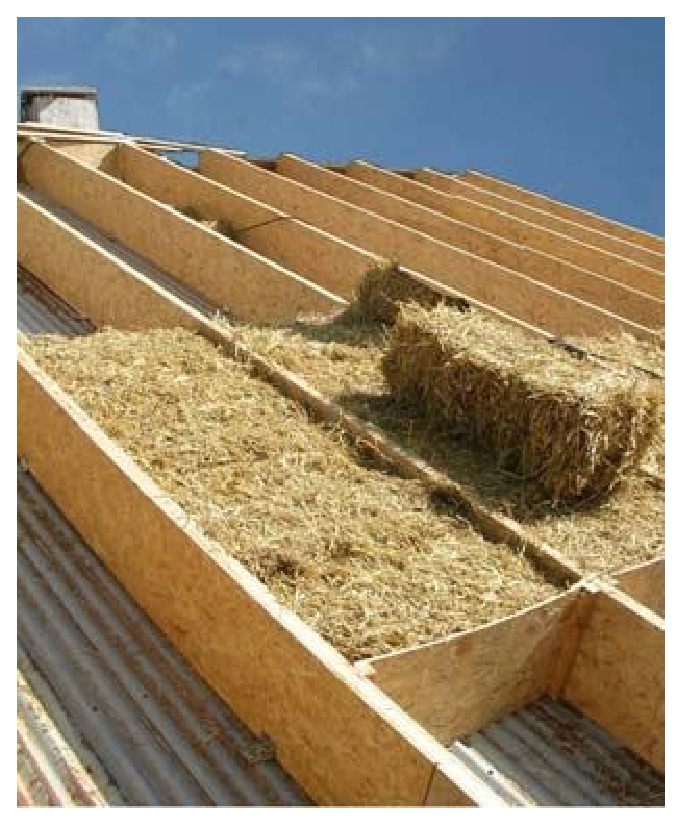
\includegraphics[width=4cm]{images-004.eps}
} 
\end{center}

Il disposera les bottes de paille sur la surface correspondant à la zone grisée, pour créer une isolation de 35~cm d'épaisseur. 

Pour calculer le nombre de bottes de paille qu'il doit commander, il considère que les bottes sont disposées les unes contre les autres. Il ne tient pas compte de l'épaisseur des planches entre lesquelles il insère les bottes. 

	\begin{enumerate}
		\item Combien de bottes devra-t-il commander ? 
		\item Quel est le coût de la paille nécessaire pour isoler le toit ? 
	\end{enumerate}
\end{enumerate}
